\scanpage{5}
\mspage{(3)}
i.e. a) $C^\bullet_{\mathrm{DRS}}(X,\mathbb Q)$ dépend de $X$ via $S_*(X)$

b) Sur $(\mathrm{Ss}\unsure{\simeq}(\mathrm{Ens})_*$, le foncteur $C^\bullet_{\mathrm{DRS}}(-,\mathbb Q)$ est représentable par $\mathrm{DRS}^\bullet_*$.

Or a) $\mathrm{DRS}^\bullet_*$ est une résolution de $\mathbb Q_*$ \inserted{(dans la cat. des groupes $\frac12$ simpl.)} (lemme de Poincaré algébrique sur les espaces \inserted{$\mathbb Q$-}affines $E^{[n]}$)

b) Les composantes $\mathrm{DRS}^i_*$ $(i\geq0)$ de $\mathrm{DRS}^\bullet_*$ sont des objets \inserted{acycliques} du topos $\mathrm{Ss}$ (ce qui revient à dire que leurs $\pi_j(\mathrm{DRS}^i_*)$ sont nuls, ce qui se vérifie facilement). [\unsure{Il en serait itou} avec des formes $C^\infty$ à coeff dans $\mathbb R$ ou $\mathbb C$, -- analytiques réelles, ou analytiques complexes...]

\deleted{\unsure{On peut prendre}}\figure{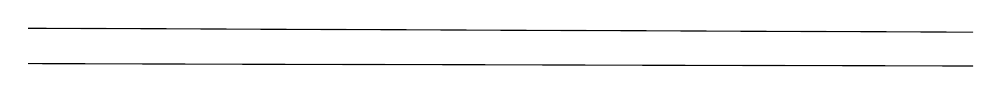
\begin{tikzpicture}\draw (0,.45)--(12,.4);\draw (0,0)--(12,-.03);\end{tikzpicture}}
\margin{On aimerait avoir une $\mathbb Z$-algèbre diff. $C^\bullet_{\mathrm{DR}}(X,\mathbb Z)$ \uline{\unsure{anticomm.}} (dépendant fonct. de $X$ par $S_*(X)$) dont la coh. soit la coh. \unsure{entière de $X$|entière avec $\mathbb Z$}. Mais il paraît qu'il y a des ths contre ! On va pourtant y arriver \deleted{\illegible{1}} \inserted{\unsure{quand même !|en un sens !}}}

Si on prend $C^\bullet_{\mathbb Z\text{-}\mathrm{DR}}(E^{[n]})$ (car $E^{[n]}$ a une $\mathbb Z$-structure affine) c'est a) qui devient déjà faux : pour intégrer $\int x^n\,dx$, il faut un dénominateur \inserted{avec $\dfrac{x^{n+1}}{n+1}$} ! Mais en géom. alg. on est déjà familiarisé avec une façon de sauter à pieds-joints \deleted{sur} \inserted{par dessus} le \unsure{caniveau}, en introduisant des p.d. et des polynômes \inserted{(ou séries formelles)} à puiss. div. Si $E^{[n]}$ avait une origine sur $\mathbb Z$ (i.e. provenant \unsure{can.} d'un $\mathbb Z$-module libre de t.f.) -- on aurait un complexe de De Rham à p.d. Mais pas pour un espace affine ! Notons
\[
\begin{aligned}
\mathrm{DRS}^\bullet_{[n]}&\simeq\deleted{\mathbb Q[X_i,dX_i]/}\ C^\bullet_{\mathrm{DR}/\mathbb Q}\left(\mathbb Q[(X_i)_{0\leq i\leq n}]/\textstyle\sum X_i-1\right)\\
&\simeq\mathbb Q[X_i,dX_i]_{0\leq i\leq n}/(\textstyle\sum X_i-1,\ \sum dX_i)\\
&\simeq\mathbb Q[X_0,\ldots,X_{n-1}][dX_0,\ldots,dX_{n-1}]
\end{aligned}
\]
\mspage{4}
